\clearpage 
\section{MC closure test for detector backgrounds}
\label{app:ClosureTest}

%\subsection{MC clusure test for the fake leptons}
\par{\bf}
\par{\bf MC clusure test for the fake leptons}

We did MC closure test to check if the estimated fake rate and the charge-flip rate are valid in the CRs where $t\overline{t}$ and $V+jets$ process are dominant.
In the test for the fake leptons, charge-flip background is estimated using OS events reweighted using the charge-flip weight.
The SS baseline lepton pair events are then selected from $t\overline{t}$ and $V+jets$ sample, weighted using matrix-method weight.
Events with SS signal lepton pair are selected to make comparison with the weighted baseline-lepton pair events.
The Matrix Method weight applied to the SS events are considered respectively, with the input-fake-rate estimated from MC and data.
Also, two regions are defined for the closure test in different $b-jet$ multiplicity, shown on Table \ref{tab:region_closure_test_fake}.
The fake-rate from MC and data are shown on Table \ref{tab:ct_fr_el} and Table \ref{tab:ct_fr_mu}.
Number of jet distribution was shown on figure Figure~\ref{fig:fake_closure_test} for the test.
Reasonable agreement is obtained in this closure test(within 10$\%$).

%------------------------------------------------
\begin{table}[!htb]
\centering
\begin{tabular}{|l|c|c|c|}
\hline
 & Leptons & Jets & MET \\
\hline \hline
0-$b$jet region      & \texttt{$\geq$2 signal lepton} &  \texttt{exactly 0 $b-jet$} & \texttt{$\geq$40GeV}  \\
                   & $p^{T}$ $>$ 10GeV & $p^{T}$$>$20GeV  & \\
\hline
1-$b$jet region      & \texttt{$\geq$2 signal lepton} &  \texttt{$\geq$1 $b-jet$} & \texttt{$\geq$40GeV}  \\
                   & $p^{T}$ $>$ 10GeV & $p^{T}$$>$20GeV  & \\
\hline
\end{tabular}
\caption{Lepton and $b-jet$s selection cuts of the region for fake closure test.}
\label{tab:region_closure_test_fake}
\end{table}
%------------------------------------------------


%------------------------------------------------
\begin{table}[!htb]
\caption{
\label{tab:ct_fr_el}
The electron fake rate used in the closure test from MC.
%\textcolor{red}{To be updated}
}
\begin{center}
\begin{tabular}{|c|c|c|}
\hline
  $p^{T}$               &                  data                   &                  MC       \\
\hline\hline
10GeV $<$ pt $<$ 20GeV  &    0.076 $\pm$ 0.014 $\pm$ 0.038       &     0.047 $\pm$ 0.001 $\pm$ 0.023  \\
 pt $>$  20GeV          &    0.118 $\pm$ 0.033 $\pm$ 0.063       &     0.046 $\pm$ 0.001 $\pm$ 0.023   \\
\hline
\hline
\end{tabular}
\end{center}
\end{table}
%------------------------------------------------

%------------------------------------------------
\begin{table}[!htb]
\caption{
\label{tab:ct_fr_mu}
The muon fake rate used in the closure test from MC.
%\textcolor{red}{To be updated}
}
\begin{center}
\begin{tabular}{|c|c|c|}
\hline
  $p^{T}$               &                  data                   &                  MC       \\
\hline\hline
10GeV $<$ pt $<$ 15GeV  &    0.187 $\pm$ 0.026 $\pm$ 0.094      &     0.131 $\pm$ 0.002 $\pm$ 0.065  \\
15GeV $<$ pt $<$ 20GeV  &    0.132 $\pm$ 0.034 $\pm$ 0.066      &     0.103 $\pm$ 0.002 $\pm$ 0.051   \\
 pt $>$  20GeV          &    0.117 $\pm$ 0.035 $\pm$ 0.059      &     0.113 $\pm$ 0.002 $\pm$ 0.056   \\
\hline
\hline
\end{tabular}
\end{center}
\end{table}
%------------------------------------------------


%------------------------------------------------
\begin{figure}[!htb]
\begin{center}
\subfigure[]{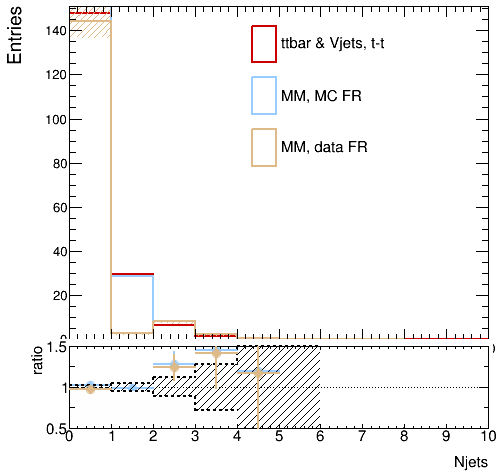
\includegraphics[width=0.4\linewidth]{BKG/closure_test/closure_test_fake_0b_njet_ee.png}}
\subfigure[]{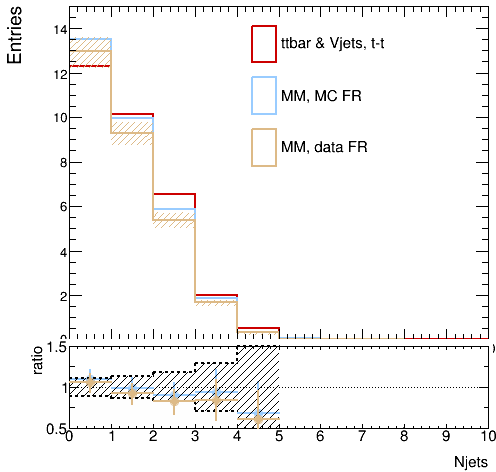
\includegraphics[width=0.4\linewidth]{BKG/closure_test/closure_test_fake_0b_njet_em.png}}
\subfigure[]{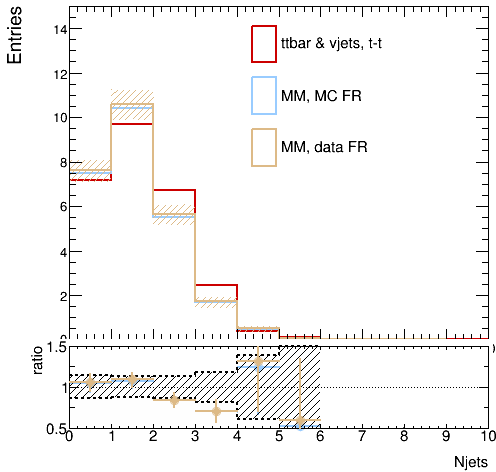
\includegraphics[width=0.4\linewidth]{BKG/closure_test/closure_test_fake_0b_njet_mm.png}}
\subfigure[]{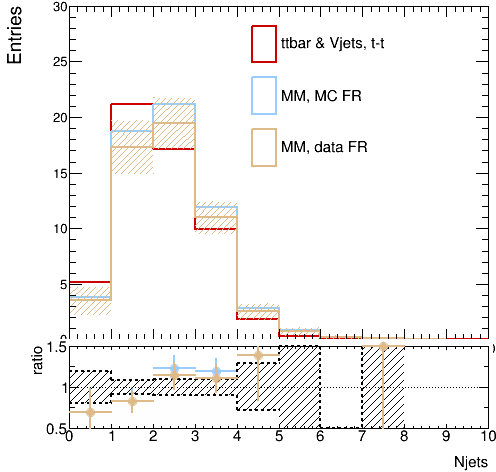
\includegraphics[width=0.4\linewidth]{BKG/closure_test/closure_test_fake_1b_njet_ee.png}}
\subfigure[]{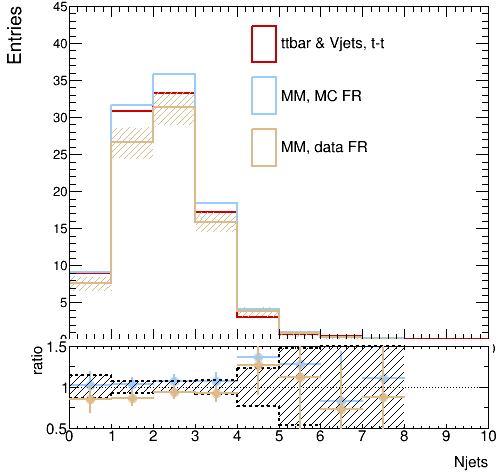
\includegraphics[width=0.4\linewidth]{BKG/closure_test/closure_test_fake_1b_njet_em.png}}
\subfigure[]{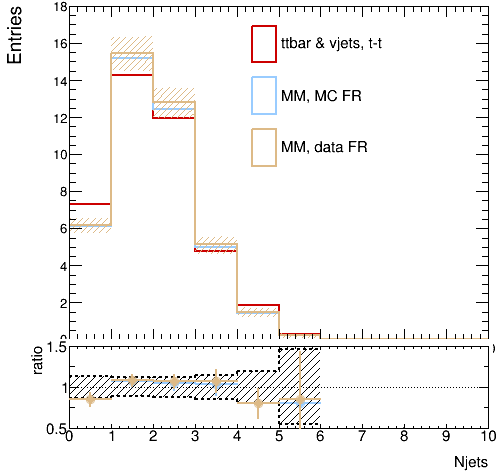
\includegraphics[width=0.4\linewidth]{BKG/closure_test/closure_test_fake_1b_njet_mm.png}}
\end{center}
\caption{\label{fig:fake_closure_test}
Distributions of number of jets for $t\overline{t}$ and $V+jets$ sample: e-e channel, region $0-bjet$ (a),
e-$\mu$ channel, region $0-bjet$ (b),
$\mu$-$\mu$ channel, region $0-bjet$ (c),
e-e channel, region $1-bjet$ (d),
e-$\mu$ channel, region $1-bjet$ (e),
$\mu$-$\mu$ channel, region $1-bjet$ (f)
Comparisons are shown among: Events with 2 same-sign leptons (red histogram);
Events with 2 same-sign baseline leptons, applying Matrix-Method weight using fake-rate from MC (blue);
Events with 2 same-sign baseline leptons, applying Matrix-Method weight usin using rate from data (golden).
}
\end{figure}
%------------------------------------------------


%\subsection{Closure test for the charge-flip}

\par{\bf Closure test for the charge-flip}

The charge-flip background should be subtracted in the fake-rate estimation.
A closure test for the subtraction is indispensable, as a validation of the charge-flip rate in $t\overline{t}$ and $V+jets$ sample.
Two regions in different $b-jet$ multiplicity was considered for the charge-flip closure test, definition shown on Table \ref{tab:region_closure_test_cf}.

%------------------------------------------------
\begin{table}[!htb]
\centering
\begin{tabular}{|l|c|c|}
\hline
 & Leptons & Jets \\
\hline \hline
0-$b$jet region      & \texttt{$\geq$2 signal lepton} &  \texttt{exactly 0 $b-jet$}   \\
                   & $p^{T}$$>$10GeV & $p^{T}$$>$20GeV  \\
\hline
1-$b$jet region      & \texttt{$\geq$2 signal lepton} &  \texttt{$\geq$1 $b-jet$}   \\
                   & $p^{T}$$>$ 10GeV & $p^{T}$$>$ 20GeV  \\
\hline
\end{tabular}
\caption{ Lepton and $b-jet$s selection cuts of the region for charge-flip closure test.}
\label{tab:region_closure_test_cf}
\end{table}
%------------------------------------------------




SS events and OS events are selected separately in the charge-flip closure test. 
The OS events are applied with charge-flip weight using rate estimated based on data or MC15 respectively.
The contribution of chage-flip lepton backround can also be estimated directly using the truth information from the SS events.
Number of jets distributions are used to perform the comparison between the two estimations of charge-flip, shown on Figure~\ref{fig:CF_closure_test}.
The SS distribution should be consistent with the OS distribution using MC charge-flip rate.
This is observed from the distribution, showing a good charge-flip subtraction in the fake-rate CR.

%------------------------------------------------
\begin{figure}[!htb]
\begin{center}
\subfigure[]{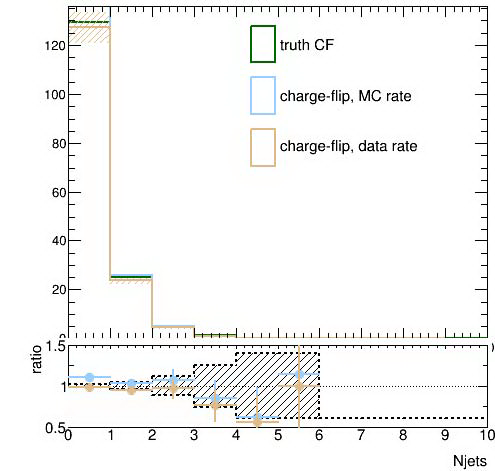
\includegraphics[width=0.45\linewidth]{BKG/closure_test/closure_test_CF_0b_njet_ee.png}}
\subfigure[]{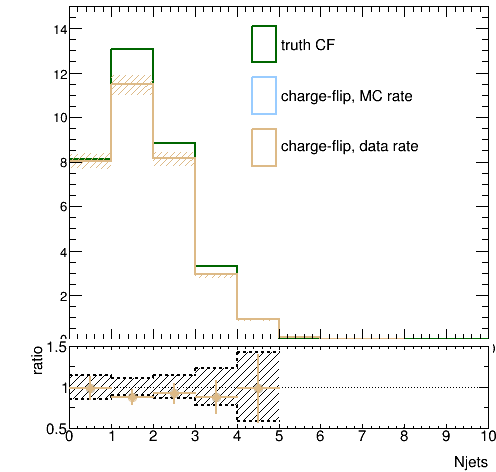
\includegraphics[width=0.45\linewidth]{BKG/closure_test/closure_test_CF_0b_njet_em.png}}
\subfigure[]{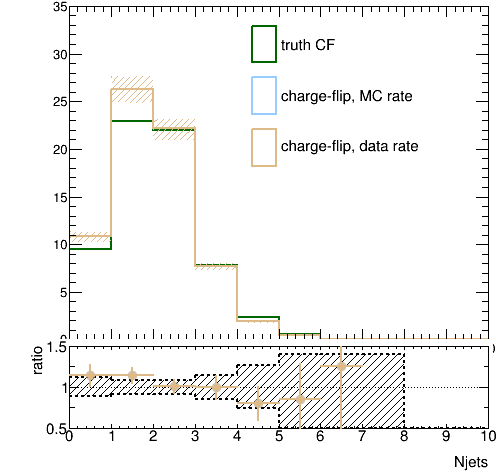
\includegraphics[width=0.45\linewidth]{BKG/closure_test/closure_test_CF_1b_njet_ee.png}}
\subfigure[]{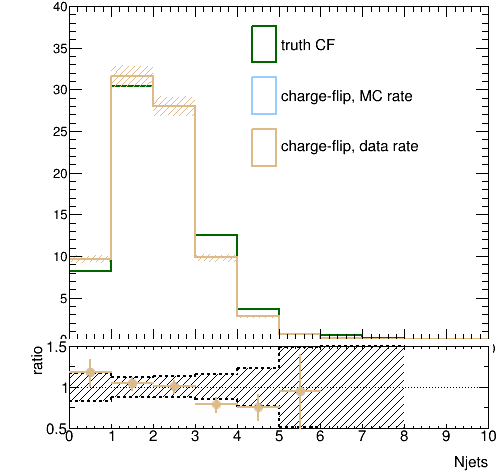
\includegraphics[width=0.45\linewidth]{BKG/closure_test/closure_test_CF_1b_njet_em.png}}
\end{center}
\caption{\label{fig:CF_closure_test}
Distributions of number of jets for $t\overline{t}$ and $V+jets$ sample: e-e channel, region 0-$b$jet (a),
e-$\mu$ channel, region 0-$b$jet (b),
e-e channel, region 1-$b$jet (c),
e-$\mu$ channel, region 1-$b$jet (d).
Comparisons are shown among: SS charge-flip events with truth selection (green histogram); 
OS events with charge-flip weight using rate from MC (blue); 
OS events with charge-flip weight using rate from data (golden).
 }
\end{figure}
%------------------------------------------------






